\documentclass[12pt,a4paper]{article}

%-----------------------------------------------------------
% Packages
%-----------------------------------------------------------
\usepackage[margin=1in]{geometry}
\usepackage{graphicx}
\usepackage{amsmath}
\usepackage{hyperref}
\usepackage{booktabs}
\usepackage{array}
\usepackage{longtable}
\usepackage{xcolor}
\usepackage{titlesec}
\usepackage{fancyhdr}
\usepackage{enumitem}
\usepackage{tikz}
\usetikzlibrary{shapes.geometric, arrows, positioning, fit, backgrounds, calc}
\usepackage[T1]{fontenc}
\usepackage[utf8]{inputenc}
\usepackage{parskip}
\usepackage[expansion=false]{microtype}
\usepackage{float}
\usepackage{tabularx}
\usepackage{multirow}
\usepackage{mdframed}

%-----------------------------------------------------------
% Colors
%-----------------------------------------------------------
\definecolor{primaryblue}{RGB}{30, 64, 175}
\definecolor{accentteal}{RGB}{0, 180, 166}
\definecolor{accentgreen}{RGB}{5, 150, 105}
\definecolor{lightgray}{RGB}{248, 249, 250}
\definecolor{darkgray}{RGB}{55, 65, 81}
\definecolor{warningred}{RGB}{185, 28, 28}

\titleformat{\section}{\Large\bfseries\color{primaryblue}}{\thesection.}{0.5em}{}[\titlerule]
\titleformat{\subsection}{\large\bfseries\color{accentteal}}{\thesubsection.}{0.5em}{}
\titleformat{\subsubsection}{\normalsize\bfseries\color{darkgray}}{\thesubsubsection.}{0.5em}{}

\pagestyle{fancy}
\fancyhf{}
\rhead{\textcolor{primaryblue}{\textit{Architecture \& Comparison}}}
\lhead{\textcolor{primaryblue}{\textbf{WN-GPT Agent}}}
\rfoot{\thepage}
\lfoot{\textcolor{darkgray}{\footnotesize WN\_GPT Research $\cdot$ \textbf{Not} the HeyDoc WellnessGPT TSE}}

\hypersetup{
    colorlinks=true,
    linkcolor=primaryblue,
    urlcolor=accentteal,
    citecolor=accentgreen,
    pdftitle={WN-GPT Agent Architecture Research},
    pdfauthor={WN\_GPT Research}
}

\begin{document}

%=============================================================================
% Title Page
%=============================================================================
\begin{titlepage}
    \centering\vspace*{1.5cm}
    {\Huge\bfseries\color{primaryblue} WN-GPT Agent}\\[0.4cm]
    {\Large\color{accentteal} Our Multi-Agent Backend --- Problem Statement, Flow, and Comparisons}\\[0.3cm]
    {\large\color{darkgray} Code: \texttt{D:\textbackslash Internship\textbackslash WN\_GPT\textbackslash Backend}}\\[0.2cm]
    {\large\color{warningred} \textbf{Not the same as} \texttt{wellnessgpt\_tse.tex} (HeyDoc WellnessGPT product)}\\[1.2cm]

    \begin{mdframed}[backgroundcolor=lightgray, linecolor=primaryblue, linewidth=1.5pt, roundcorner=5pt]
        \centering\vspace{0.4cm}
        \textbf{This document describes \emph{our agent} (internship implementation).}\\[0.2cm]
        \textbf{External comparators:} Hippocratic AI, August AI\\
        \textbf{Related (separate) research files:}\\
        \texttt{wellnessgpt\_tse.tex} = HeyDoc commercial WellnessGPT\\
        \texttt{our\_agent.tex} = Wellbeing (WB-001) requirements vision\\
        \vspace{0.3cm}
        \textit{Our roadmap: page-indexed retrieval to reduce hallucination and provide auditable guidance.}
        \vspace{0.4cm}
    \end{mdframed}

    \vfill
    \begin{tabular}{ll}
        \textbf{Document:}   & WN-GPT Agent architecture research \\
        \textbf{Codebase:} & \texttt{Backend/} --- FastAPI + LangGraph + SQLite \\
        \textbf{Date:}     & May 2026 \\
        \textbf{Version:}  & 1.1 \\
    \end{tabular}
\end{titlepage}

\tableofcontents
\newpage

%=============================================================================
% Abstract
%=============================================================================
\begin{abstract}
\noindent
This document describes \textbf{our agent}---the WN\_GPT healthcare backend at \texttt{Backend/}---not the commercial \textbf{WellnessGPT} platform documented in \texttt{wellnessgpt\_tse.tex} (HeyDoc AI). Our implementation is a \textbf{15-agent}, \textbf{LangGraph} system with \textbf{Azure OpenAI}, \textbf{SQLite}, and a \textbf{supervisor router} (\texttt{detect\_intent}), not HeyDoc's advertised \textbf{Agentic Orchestration Engine} or \textbf{HealthMem} stack. We state the problem, document the real process flow, contrast our agent with \textbf{Hippocratic AI} and \textbf{August AI}, and specify \textbf{page-indexed grounding} as our planned anti-hallucination layer.
\end{abstract}

\newpage

%=============================================================================
\section{Three Different Systems --- Do Not Conflate}
%=============================================================================

Three LaTeX artifacts in \texttt{Research/} refer to \emph{related but distinct} systems. Treating them as one product causes incorrect architecture claims.

\begin{table}[H]
\centering
\renewcommand{\arraystretch}{1.4}
\small
\begin{tabularx}{\textwidth}{@{}p{2.6cm}p{3.2cm}p{4.2cm}p{4.5cm}@{}}
\toprule
\textbf{Name} & \textbf{File} & \textbf{What it is} & \textbf{Key architecture (claimed or built)} \\
\midrule
\textbf{WellnessGPT} (HeyDoc) &
\texttt{wellnessgpt\_tse.tex} &
Commercial / marketing TSE for HeyDoc AI (wellness-gpt.com, HeyDoc app) &
Three pillars: 15+ agents, \textbf{Agentic Orchestration Engine}, \textbf{HealthMem} (vector + graph + KV), HIPAA/FHIR/ABDM enterprise SaaS \\

\textbf{Wellbeing} (WB-001) &
\texttt{our\_agent.tex} &
Software requirements / vision spec for a clinical Agentic OS &
Hybrid \textbf{RAG-first} (Neo4j + Pinecone), LangGraph orchestrator, evidence panels, Epic/Cerner FHIR --- \textbf{target design}, not identical to code \\

\textbf{WN-GPT Agent} (\textbf{ours}) &
\texttt{Backend/} + \textbf{this document} &
Internship implementation you run locally &
LangGraph \textbf{supervisor router} (no orchestrator LLM), 15 ReAct agents, \textbf{SQLite} only, local uploads; \textbf{no} HealthMem, \textbf{no} Neo4j/Pinecone in repo \\
\bottomrule
\end{tabularx}
\caption{WellnessGPT (HeyDoc TSE) $\neq$ Wellbeing SRS $\neq$ WN-GPT Backend (our agent)}
\end{table}

\begin{mdframed}[backgroundcolor=lightgray, linecolor=warningred, linewidth=1pt]
\textbf{Rule for readers:} When this repository says ``WellnessGPT'' in \texttt{main.py} or CLI branding, it is a \emph{working title} for the demo backend. For research and comparisons, use \textbf{WN-GPT Agent} for our code and reserve \textbf{WellnessGPT} for \texttt{wellnessgpt\_tse.tex} unless explicitly discussing HeyDoc's product roadmap.
\end{mdframed}

\subsection{What Our Agent Actually Implements vs.\ HeyDoc WellnessGPT TSE}

\begin{table}[H]
\centering
\renewcommand{\arraystretch}{1.35}
\begin{tabularx}{\textwidth}{lcc}
\toprule
\textbf{Capability} & \textbf{wellnessgpt\_tse.tex} & \textbf{WN-GPT Agent (Backend/)} \\
\midrule
Orchestration & Full Agentic Orchestration Engine; multi-step agent handoffs & \texttt{detect\_intent} + single agent per message; no handoffs \\
Memory & HealthMem (vector + graph + KV, sub-150ms recall) & SQLite tables + JSON fields; no vector DB \\
Compliance story & HIPAA, FHIR, ABDM production framing & Demo \texttt{X-Patient-ID} auth; ABDM stub \\
RAG / evidence & Enterprise knowledge + EHR connectors & Tool calls to SQLite; page index \textbf{planned} \\
CLI / API & Enterprise deployment narrative & FastAPI + Rich CLI (CLI skips agent tools) \\
\bottomrule
\end{tabularx}
\caption{Our agent is an early \emph{prototype} of specialist routing, not the full HeyDoc WellnessGPT platform}
\end{table}

\newpage

%=============================================================================
\section{Problem Statement (WN-GPT Agent)}
%=============================================================================

\subsection{Clinical and Operational Context}

Healthcare organizations need AI that can support patients and staff across \emph{many} workflows---triage, scheduling, pharmacy, insurance, nutrition, mental health, and hospital operations---without treating every question as a generic chat. Single-model chatbots fail because they lack persistent patient context, domain-specific tools, and traceable evidence for clinical statements.

\subsection{Core Problems Addressed by Our Agent}

\begin{enumerate}[leftmargin=*]
    \item \textbf{Fragmented patient journeys.} Users repeat symptoms, medications, and history across channels; there is no unified agent layer that routes requests to the correct clinical or administrative specialist.
    \item \textbf{Hallucination in medical answers.} Large language models can produce confident but incorrect dosing, contraindication, or triage advice when not grounded in patient records or source documents.
    \item \textbf{Lack of structured workflow execution.} Healthcare tasks (book appointment, log triage, file claim) require database writes and JSON-structured outputs, not free-form prose alone.
    \item \textbf{India-specific interoperability.} Systems must align with ABHA/ABDM health records and local hospital operations, not only US-centric EHR copilots.
    \item \textbf{Auditability and safety.} Clinicians and patients need to know \emph{which agent} answered, \emph{what data} was used, and \emph{which document page} supports a recommendation.
\end{enumerate}

\subsection{Research Question}

\begin{quote}
\textit{How can a multi-agent healthcare platform combine intent-based routing, tool-grounded specialists, and page-indexed retrieval to deliver safer, more explainable guidance than monolithic consumer health chatbots?}
\end{quote}

\subsection{Scope of This Document}

\begin{itemize}[noitemsep]
    \item \textbf{In scope:} Backend at \texttt{Backend/} (API, LangGraph, agents, SQLite, CLI).
    \item \textbf{Out of scope:} Frontend UI, production HIPAA certification, live ABDM production APIs (stubs exist).
    \item \textbf{Planned (design):} Full page-index pipeline for uploaded PDFs and clinical corpora.
\end{itemize}

\newpage

%=============================================================================
\section{WN-GPT Backend Architecture (Our Implementation)}
%=============================================================================

\subsection{Repository Layout}

\begin{table}[H]
\centering
\renewcommand{\arraystretch}{1.3}
\begin{tabularx}{\textwidth}{lX}
\toprule
\textbf{Path} & \textbf{Role} \\
\midrule
\texttt{main.py} & FastAPI entry; CORS; auth middleware; mounts \texttt{/api/v1} routers \\
\texttt{app/core/graph\_factory.py} & Compiles LangGraph: intent node + 15 agents + utilities \\
\texttt{app/services/routing.py} & \texttt{detect\_intent} (keywords + LLM) and \texttt{route\_to\_agent} \\
\texttt{app/services/agents/} & One Python module per specialist (ReAct + tools) \\
\texttt{app/db/repository.py} & SQLite CRUD (patients, triage, care plans, etc.) \\
\texttt{app/schemas/state.py} & Shared \texttt{AgentState} TypedDict for all nodes \\
\texttt{cli/} & Rich terminal UI; streaming demo (no LangGraph tools) \\
\texttt{db\_init/} & Schema + seed SQL $\rightarrow$ \texttt{wellness.db} \\
\bottomrule
\end{tabularx}
\caption{WN-GPT Agent backend structure (\texttt{D:\textbackslash Internship\textbackslash WN\_GPT\textbackslash Backend})}
\end{table}

\subsection{Technology Stack}

\begin{itemize}[noitemsep]
    \item \textbf{API:} FastAPI, Uvicorn, \texttt{X-Patient-ID} demo authentication
    \item \textbf{Orchestration:} LangGraph \texttt{StateGraph}, single-hop routing (no multi-agent chains)
    \item \textbf{LLM:} Azure OpenAI (e.g.\ GPT-4o) via LangChain
    \item \textbf{Agents:} \texttt{create\_react\_agent} with repository-backed \texttt{@tool} functions
    \item \textbf{Data:} SQLite (\texttt{wellness.db}); local \texttt{uploads/} for documents
\end{itemize}

\subsection{Fifteen Specialist Agents}

\begin{longtable}{@{}p{3.2cm}p{4.2cm}p{7.5cm}@{}}
\toprule
\textbf{Intent key} & \textbf{Graph node} & \textbf{Primary function} \\
\midrule
\endhead
\texttt{triage} & \texttt{triage\_agent} & Symptom urgency, specialty, emergency flag; logs to \texttt{symptoms\_logs} \\
\texttt{booking} & \texttt{booking\_agent} & Appointment scheduling, doctor slots \\
\texttt{channeling} & \texttt{channeling\_agent} & Symptom $\rightarrow$ specialty routing \\
\texttt{adherence} & \texttt{adherence\_agent} & Medication follow-up, reminders \\
\texttt{care\_plan} & \texttt{care\_manager\_agent} & Preventive care, wellness plans \\
\texttt{discharge} & \texttt{discharge\_agent} & Discharge summaries and instructions \\
\texttt{insurance} & \texttt{insurance\_agent} & Coverage, claims, billing gaps \\
\texttt{hospital\_ops} & \texttt{hospital\_ops\_agent} & Beds, inventory, ward status \\
\texttt{pharmacy} & \texttt{pharmacy\_agent} & Prescriptions, interactions, refills \\
\texttt{mental\_health} & \texttt{mental\_health\_agent} & PHQ-9/GAD-7 screening, risk, escalation \\
\texttt{family\_care} & \texttt{family\_care\_agent} & Household-level health aggregation \\
\texttt{product\_rec} & \texttt{product\_rec\_agent} & Catalog-backed product suggestions \\
\texttt{report\_analysis} & \texttt{report\_analyzer\_agent} & Lab/PDF report interpretation \\
\texttt{nutrisense} & \texttt{nutrisense\_agent} & Diet plans, nutrition logs \\
\texttt{fitguide} & \texttt{fitguide\_agent} & Exercise plans, fitness logs \\
\midrule
\texttt{health\_records} & \texttt{health\_records\_node} & ABDM/ABHA record pull (stub) \\
\texttt{general} & \texttt{general\_response} & Fallback conversational LLM \\
\bottomrule
\caption{Agent registry in \texttt{graph\_factory.py} (15 ReAct specialists + 2 utility nodes)}
\end{longtable}

\newpage

%=============================================================================
\section{Agent Process Flow}
%=============================================================================

\subsection{Supervisor Routing (Not an Orchestrator Agent)}

Our WN-GPT agent does \textbf{not} use HeyDoc's ``Agentic Orchestration Engine'' nor a separate orchestrator LLM. It uses a \textbf{supervisor router} (\texttt{detect\_intent}) that dispatches to exactly \textbf{one} specialist per user message---simpler than the multi-agent workflows described in \texttt{wellnessgpt\_tse.tex}.

\begin{figure}[H]
\centering
\begin{tikzpicture}[
    node distance=1.4cm,
    block/.style={rectangle, draw=primaryblue, fill=primaryblue!8, rounded corners,
                  minimum width=9em, minimum height=2.6em, align=center, font=\small},
    decision/.style={diamond, draw=accentteal, fill=accentteal!12, aspect=2.2,
                     inner sep=1pt, align=center, font=\small},
    arrow/.style={-{Stealth[length=2.2mm]}, thick, primaryblue}
]
    \node[block] (user) {User message\\(API or CLI)};
    \node[block, below=of user] (detect) {\texttt{detect\_intent}};
    \node[decision, below=of detect] (route) {Route};
    \node[block, below left=1.2cm and 0.8cm of route] (agent) {One specialist\\agent node};
    \node[block, below right=1.2cm and 0.8cm of route] (util) {Health records /\\General fallback};
    \node[block, below=2.2cm of route] (end) {\texttt{agent\_response}};

    \draw[arrow] (user) -- (detect);
    \draw[arrow] (detect) -- (route);
    \draw[arrow] (route) -| (agent);
    \draw[arrow] (route) -| (util);
    \draw[arrow] (agent) |- (end);
    \draw[arrow] (util) |- (end);
\end{tikzpicture}
\caption{High-level LangGraph flow: single intent, single agent, then END}
\end{figure}

\subsection{Intent Detection Algorithm}

\texttt{detect\_intent} in \texttt{routing.py} uses a \textbf{hybrid} strategy:

\begin{enumerate}[noitemsep]
    \item \textbf{Keyword pass} on the last user message (16 intent buckets: pain $\rightarrow$ triage, diet $\rightarrow$ nutrisense, etc.).
    \item \textbf{LLM fallback} if no keyword matches: Azure OpenAI classifies into one intent name only.
    \item \textbf{Normalization} via \texttt{normalize\_enum} to reject invalid LLM labels.
\end{enumerate}

\subsection{Per-Agent Micro-Flow (API Path)}

Each specialist agent follows the same ReAct pattern:

\begin{figure}[H]
\centering
\begin{tikzpicture}[
    node distance=1.1cm,
    step/.style={rectangle, draw=accentgreen, fill=accentgreen!10, rounded corners,
                minimum width=11em, minimum height=2.2em, align=center, font=\small},
    arrow/.style={-{Stealth[length=2mm]}, thick, accentgreen}
]
    \node[step] (s1) {System prompt + JSON schema};
    \node[step, below=of s1] (s2) {ReAct loop: LLM $\leftrightarrow$ tools};
    \node[step, below=of s2] (s3) {Tools: \texttt{repository} (SQLite)};
    \node[step, below=of s3] (s4) {Parse JSON $\rightarrow$ update \texttt{AgentState}};
    \node[step, below=of s4] (s5) {Return \texttt{agent\_response}};

    \foreach \a/\b in {s1/s2, s2/s3, s3/s4, s4/s5}
        \draw[arrow] (\a) -- (\b);
\end{tikzpicture}
\caption{Inside one specialist agent (e.g.\ NutriSense, Triage, Pharmacy)}
\end{figure}

\textbf{Example tools:} \texttt{get\_patient}, \texttt{get\_triage\_history}, \texttt{save\_triage\_result}, \texttt{get\_nutrition\_context}, \texttt{save\_nutrition\_plan}.

\subsection{API vs CLI Paths}

\begin{table}[H]
\centering
\renewcommand{\arraystretch}{1.4}
\begin{tabularx}{\textwidth}{lXX}
\toprule
\textbf{Aspect} & \textbf{API (\texttt{POST /api/v1/chat/})} & \textbf{CLI (\texttt{python -m cli})} \\
\midrule
Orchestration & Full LangGraph \texttt{graph.invoke} & \texttt{detect\_intent} only \\
Agent tools   & Yes (SQLite via ReAct) & No \\
Output        & JSON \texttt{ChatResponse} & Rich streaming terminal \\
Patient auth  & \texttt{X-Patient-ID} header & \texttt{--patient P001} \\
\bottomrule
\end{tabularx}
\caption{Dual interfaces---research comparisons should use the API path for agent fidelity}
\end{table}

\subsection{Structured Data Side-Channels}

Forms can bypass the graph and write directly to SQLite:

\begin{itemize}[noitemsep]
    \item \texttt{POST /patient/\{id\}/symptoms}, \texttt{/nutrition}, \texttt{/fitness}, \texttt{/mental-health}
    \item \texttt{POST /patient/\{id\}/upload} $\rightarrow$ local storage + \texttt{patient\_documents}
\end{itemize}

\newpage

%=============================================================================
\section{Page-Indexed Grounding for Hallucination Reduction}
%=============================================================================

\subsection{Motivation}

Keyword routing and SQLite tools reduce \emph{wrong-agent} errors and \emph{fabricated patient facts}, but they do not fully solve \textbf{document hallucination}---inventing lab values, misreading PDF tables, or citing non-existent guidelines. Consumer platforms (e.g.\ August AI) store reports in memory; enterprise voice agents (e.g.\ Hippocratic AI) use multi-model safety constellations; HeyDoc's WellnessGPT TSE describes HealthMem + orchestration. \textbf{Our agent} proposes a complementary, implementable strategy: \textbf{page-indexed retrieval} on uploaded clinical PDFs (aligned with the RAG vision in \texttt{our\_agent.tex}, but not yet built).

\subsection{Page Indexing Concept}

\begin{mdframed}[backgroundcolor=lightgray, linecolor=accentteal, linewidth=1pt]
\textbf{Page index:} A structured map from each logical page (or section) of a clinical document to retrievable text, tables, figures, and metadata (document ID, page number, bounding region). Agents must cite \texttt{(doc\_id, page, span)} when stating facts from uploads or corpora.
\end{mdframed}

\begin{enumerate}[leftmargin=*]
    \item \textbf{Ingestion:} User uploads PDF/image via \texttt{/patient/\{id\}/upload} $\rightarrow$ stored under \texttt{uploads/}.
    \item \textbf{Indexing:} Build a \emph{pageindex} artifact: per-page text blocks, table HTML, figure paths (analogous to canonical bundle + pageindex pipelines used in document-AI systems).
    \item \textbf{Retrieval:} On \texttt{report\_analysis}, \texttt{pharmacy}, or \texttt{nutrisense} intents, fetch only top-$k$ \textbf{pages} (not whole-document dumps) relevant to the query.
    \item \textbf{Generation:} ReAct agent receives retrieved pages as context; system prompt requires answers to include \textbf{page references} and ``insufficient evidence'' when retrieval is empty.
    \item \textbf{Guidance layer:} Map retrieved spans to patient-specific constraints (allergies, chronic conditions from SQLite) before final natural-language guidance.
\end{enumerate}

\subsection{Current vs Planned Implementation}

\begin{table}[H]
\centering
\renewcommand{\arraystretch}{1.35}
\begin{tabularx}{\textwidth}{lcc}
\toprule
\textbf{Capability} & \textbf{Current backend} & \textbf{With page indexing} \\
\midrule
Patient profile grounding & Yes (SQLite tools) & Yes \\
Intent routing            & Yes (keywords + LLM) & Yes \\
Document upload storage   & Yes (\texttt{uploads/}) & Yes \\
Per-page index artifacts  & No & Yes (planned) \\
Citation in agent output  & No & Yes (planned) \\
Vector / semantic search  & No & Optional hybrid with page filter \\
Report OCR                & Stub/simulated & Real pipeline + page map \\
\bottomrule
\end{tabularx}
\caption{Anti-hallucination layers: implemented today vs page-index roadmap}
\end{table}

\subsection{Why Page Indexing Reduces Hallucination}

\begin{itemize}[noitemsep]
    \item \textbf{Bounded context:} LLM sees only retrieved pages, not entire 200-page PDFs (reduces confabulation from noise).
    \item \textbf{Verifiable citations:} UI can show ``Page 3, Table 2'' for clinician verification.
    \item \textbf{Deterministic anchors:} Tool calls return exact stored spans; model paraphrases \emph{after} retrieval.
    \item \textbf{Agent-specific indexes:} NutriSense indexes dietary guidelines; Report Analyzer indexes lab PDFs; Pharmacy indexes prescription leaflets---each agent queries its allowed corpus.
\end{itemize}

\newpage

%=============================================================================
\section{Comparative Analysis}
%=============================================================================

\subsection{Platform Summaries}

\textbf{Hippocratic AI} (USA, founded 2023) deploys \textbf{patient-facing voice agents} for chronic care outreach, intake, and administrative tasks. Its \textbf{Polaris constellation} uses a primary conversational model plus many specialized \textbf{safety engines} (overdose checks, escalation, medication reconciliation). Validation emphasizes \textbf{Real-World Evaluation (RWE-LLM)} with licensed clinicians reviewing outputs at scale.

\textbf{August AI} (India/global, founded 2022) is a \textbf{consumer health companion} (mobile app, WhatsApp) offering symptom guidance, secure storage of lab reports, and personalized tracking. It reports large user scale and Azure OpenAI infrastructure; it is \textbf{not} positioned as a 15-agent hospital OS but as a 24/7 personal health assistant.

\textbf{WN-GPT Agent} (our \texttt{Backend/}) is a \textbf{multi-agent LangGraph prototype} with 15 domain specialists, SQLite patient data, India-relevant ABDM stubs, and a planned \textbf{page-indexed} grounding layer. It is \textbf{not} the HeyDoc WellnessGPT enterprise platform from \texttt{wellnessgpt\_tse.tex}.

\subsection{Comparison Table}

\begin{table}[H]
\centering
\footnotesize
\renewcommand{\arraystretch}{1.45}
\begin{tabularx}{\linewidth}{@{}p{2.4cm}XXX@{}}
\toprule
\textbf{Dimension} & \textbf{Hippocratic AI} & \textbf{August AI} & \textbf{WN-GPT Agent (ours)} \\
\midrule
Primary user & Health systems, care teams & Individual consumers & Internship/demo; patients via API \\
Interaction mode & Voice-first outbound/inbound & Chat, app, WhatsApp & REST API + Rich CLI \\
Agent architecture & Polaris multi-model constellation & Monolithic / unified companion & 15 LangGraph ReAct specialists \\
Routing & Internal safety + task models & Intent within single product & \texttt{detect\_intent} supervisor router \\
Memory & Call + EHR context & Long-term user memory, reports & SQLite only (not HealthMem) \\
Grounding strategy & Many safety classifier models & Stored labs + conversation history & Tool SQL + \textbf{page-indexed docs (planned)} \\
Hallucination control & RWE-LLM, clinician review & Disclaimers; symptom checker & JSON schemas, tools, page cites (planned) \\
Clinical scope & Non-diagnostic outreach, admin & General wellness guidance & Triage, ops, insurance, nutrition, etc. \\
India / ABDM & US-focused & Strong India presence & ABHA/ABDM stub \\
Open backend & Proprietary enterprise & Proprietary consumer & \texttt{WN\_GPT/Backend} (this repo) \\
\bottomrule
\end{tabularx}
\caption{Hippocratic AI vs August AI vs \textbf{our} WN-GPT Agent (not HeyDoc WellnessGPT TSE)}
\end{table}

\subsection{Process Flow Comparison}

\begin{figure}[H]
\centering
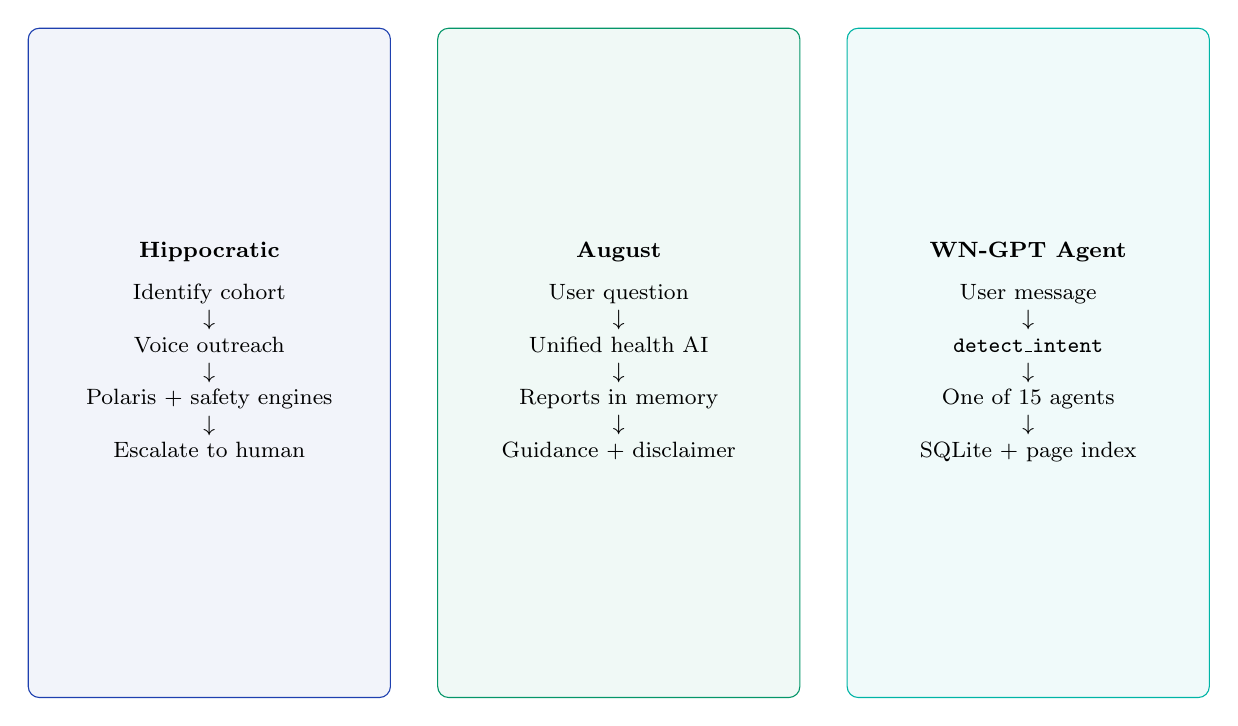
\begin{tikzpicture}[
    col/.style={rectangle, draw, minimum width=4.6cm, minimum height=8.5cm, rounded corners, align=center, font=\footnotesize},
    hippo/.style={col, draw=primaryblue, fill=primaryblue!6},
    august/.style={col, draw=accentgreen, fill=accentgreen!6},
    well/.style={col, draw=accentteal, fill=accentteal!6}
]
    \node[hippo] (h) at (0,0) {
        \textbf{Hippocratic}\\[2mm]
        Identify cohort\\
        $\downarrow$\\
        Voice outreach\\
        $\downarrow$\\
        Polaris + safety engines\\
        $\downarrow$\\
        Escalate to human\\
    };
    \node[august] (a) at (5.2,0) {
        \textbf{August}\\[2mm]
        User question\\
        $\downarrow$\\
        Unified health AI\\
        $\downarrow$\\
        Reports in memory\\
        $\downarrow$\\
        Guidance + disclaimer\\
    };
    \node[well] (w) at (10.4,0) {
        \textbf{WN-GPT Agent}\\[2mm]
        User message\\
        $\downarrow$\\
        \texttt{detect\_intent}\\
        $\downarrow$\\
        One of 15 agents\\
        $\downarrow$\\
        SQLite + page index\\
    };
\end{tikzpicture}
\caption{Simplified operational flows (conceptual)}
\end{figure}

\subsection{Strategic Positioning (Our Agent)}

\begin{itemize}[leftmargin=*]
    \item \textbf{vs Hippocratic AI:} Our agent prototypes broader in-app workflows (beds, insurance, nutrisense), not voice outreach; page indexing targets document verifiability with explicit page citations.
    \item \textbf{vs August AI:} Our agent trades consumer simplicity for specialist routing and hospital ops APIs; page-indexed retrieval is the planned answer to lab-report grounding.
    \item \textbf{vs HeyDoc WellnessGPT (\texttt{wellnessgpt\_tse.tex}):} HeyDoc describes enterprise orchestration + HealthMem; we implement a \textbf{minimal viable} multi-agent router in SQLite as a step toward that vision.
    \item \textbf{vs Wellbeing SRS (\texttt{our\_agent.tex}):} WB-001 specifies Neo4j/Pinecone RAG; our code is the \textbf{first engineering slice}---LangGraph agents + planned page index instead of full hybrid memory.
    \item \textbf{Our thesis:} Specialist agents + supervisor routing + page-indexed evidence $\rightarrow$ safer guidance without claiming HealthMem or full orchestration yet.
\end{itemize}

\newpage

%=============================================================================
\section{Conclusion and Future Work}
%=============================================================================

\subsection{Summary}

The \textbf{WN-GPT Agent} backend implements a \textbf{15-agent}, \textbf{single-hop LangGraph} architecture with hybrid intent detection and SQLite-grounded ReAct tools. It is \textbf{not} the HeyDoc WellnessGPT platform in \texttt{wellnessgpt\_tse.tex} (no HealthMem, no enterprise orchestration engine). Recommended evolution: \textbf{page-indexed retrieval} on \texttt{report\_analyzer\_agent}, pharmacy, and nutrisense, with mandatory page citations---bridging toward the Wellbeing RAG vision in \texttt{our\_agent.tex}.

\subsection{Future Work}

\begin{enumerate}[noitemsep]
    \item Implement pageindex builder for \texttt{patient\_documents} uploads.
    \item Add retrieval tools: \texttt{search\_pages(query, doc\_id, k)} to agent toolkits.
    \item Extend CLI to invoke LangGraph (parity with API).
    \item Profile update API (allergies, conditions) with audit log.
    \item Replace ABDM/OCR stubs with production connectors.
    \item Evaluate hallucination rate with/without page index on held-out lab PDFs.
\end{enumerate}

\subsection{References}

\begin{itemize}[noitemsep]
    \item Hippocratic AI --- Polaris, Safety, RWE-LLM: \url{https://hippocraticai.com}
    \item August AI --- \url{https://www.meetaugust.ai}
    \item HeyDoc WellnessGPT TSE (separate product doc): \texttt{wellnessgpt\_tse.tex}
    \item Wellbeing WB-001 SRS (requirements vision): \texttt{our\_agent.tex}
    \item \textbf{Our implementation:} \texttt{D:\textbackslash Internship\textbackslash WN\_GPT\textbackslash Backend}
\end{itemize}

\end{document}
